\documentclass[aspectratio=169,11pt]{beamer}
\usepackage[T1]{fontenc}
\usepackage[utf8]{inputenc}
\usepackage{lmodern,amsmath,amssymb,graphicx,tikz}
\usetikzlibrary{arrows.meta,calc}
\usetheme{default}
\usefonttheme{serif}
\setbeamercolor{normal text}{fg=black,bg=white}
\setbeamercolor{structure}{fg=black}
\setbeamercolor{frametitle}{fg=black}
\setbeamercolor{title}{fg=black}
\setbeamertemplate{navigation symbols}{}
\setbeamertemplate{footline}[frame number]
\setbeamertemplate{itemize items}[circle]
\setbeamersize{text margin left=8mm,text margin right=8mm}
\setlength{\parskip}{5pt}
\newcommand{\cO}{\mathcal O}
\newcommand{\cI}{\mathcal I}
\newcommand{\cA}{\mathcal A}
\newcommand{\db}{\bar\partial}
\newcommand{\C}{\mathbb C}
\newcommand{\Pj}{\mathbb P}
\newcommand{\norm}[1]{\lVert#1\rVert}
\newcommand{\src}[1]{\par\vfill{\scriptsize #1\par}}
\author{Daniel Gonz\'alez Casanova Azuela}

\title{Kodaira embedding through vanishing}
\subtitle{Lecture 24: the metrics and Kawamata--Viehweg}
\date{Hodge theory}
\begin{document}
\begin{frame}\titlepage\end{frame}
\begin{frame}{Where we left off}
For \(A=L^N\), vanishing of \(H^1(X,A\otimes I)\) lets us prescribe:
\[
\begin{array}{c|c}
I&\text{data}\\ \hline
\mathfrak m_x&\text{one value}\\
\mathfrak m_x\cap\mathfrak m_y&\text{two values}\\
\mathfrak m_x^2&\text{first jets}
\end{array}
\]
Lecture 23 (Daniel) reduced embedding to constructing positive metrics on
\[
B_N=L^N\otimes K_X^{-1}
\]
with these multiplier ideals.
\end{frame}

\begin{frame}{Today's remaining steps}
\begin{enumerate}
\setlength{\itemsep}{16pt}
\item Construct the logarithmic metrics and finish Kodaira embedding.
\item Weaken positivity to nef and big.
\item Use a mild divisor metric and Nadel to prove Kawamata--Viehweg.
\end{enumerate}
\end{frame}

\begin{frame}{The singularity is local}
\begin{columns}[c]
\column{.44\textwidth}
\centering
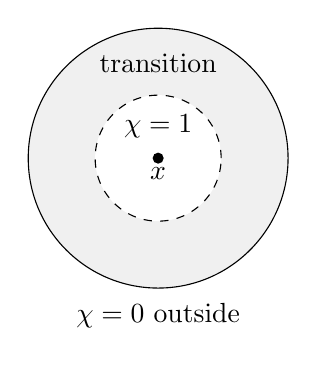
\begin{tikzpicture}[scale=1]
\fill[gray!12] (0,0) circle (1.65);
\fill[white] (0,0) circle (.8);
\draw (0,0) circle (1.65);
\draw[dashed] (0,0) circle (.8);
\fill (0,0) circle (2pt) node[below] {\(x\)};
\node at (0,.4) {\(\chi=1\)};
\node at (0,1.2) {transition};
\node at (0,-2) {\(\chi=0\) outside};
\end{tikzpicture}
\column{.53\textwidth}
Add the weight
\[
\psi_x=a\chi(z)\log|z|.
\]
Near \(x\), it gives
\[
\begin{aligned}
a=n &: \ \cI_h=\mathfrak m_x,\\[5pt]
a=n+1 &: \ \cI_h=\mathfrak m_x^2.
\end{aligned}
\]
\end{columns}
\end{frame}

\begin{frame}{Positive powers absorb the curvature loss}
Fix smooth metrics on \(L\) and \(K_X^{-1}\).
For the modified metric on \(B_N\),
\[
i\Theta_h
=N\,i\Theta_L+i\Theta_{K_X^{-1}}+2i\partial\db\psi_x.
\]
Since \(i\Theta_L\ge c\omega\), with \(c>0\),
\[
\boxed{i\Theta_h\ge(Nc-C)\omega>0\quad\text{for large }N.}
\]
The cutoff contributes only a bounded negative error.
\end{frame}

\begin{frame}{One exponent for all the prescriptions}
At \(x\), use coefficient \(n\) for \(\mathfrak m_x\), and \(n+1\) for \(\mathfrak m_x^2\).
For distinct \(x,y\), add their coefficient-\(n\) weights:
\[
\psi=\psi_x+\psi_y,\qquad
\cI_h=\mathfrak m_x\cap\mathfrak m_y.
\]
A finite coordinate cover gives uniform curvature-error bounds.
\par\bigskip
The supports may overlap. Their lower curvature bounds simply add, so one large \(N\) works for every point and pair.
\end{frame}

\begin{frame}{Kodaira embedding: conclusion}
A finite coordinate cover gives a uniform bound on all cutoff errors.
One sufficiently large \(N\) works for every point and pair.
\par\bigskip
\par The resulting \(\Phi_N\) is everywhere defined, injective, and an immersion.
\[
\boxed{X\ \text{compact}\quad\Longrightarrow\quad
\Phi_N:X\hookrightarrow\Pj^M\ \text{is an embedding}.}
\]
Conversely, the restricted Fubini--Study metric is positive.
\end{frame}

\begin{frame}{A historical pause}
Kodaira received the Fields Medal in 1954, the first Japanese recipient.
\par\bigskip
\par His vanishing theorem is a striking link between harmonic analysis and algebraic geometry.
\[
\text{positive curvature}\quad\Longrightarrow\quad
\text{enough sections to embed }X.
\]
\src{Institute for Advanced Study, scholar profile: Kunihiko Kodaira.}
\end{frame}

\begin{frame}{Nef and big}
Now let \(X\) be smooth projective, of dimension \(n\).
\par\bigskip
\par \textbf{Nef:} \(L\cdot C=\deg(L|_C)\ge0\) for every irreducible curve \(C\).
\par\bigskip
\par \textbf{Big:}
\[
\limsup_{m\to\infty}\frac{h^0(X,L^m)}{m^n}>0.
\]
There are many sections, though the bundle need not be ample.
\end{frame}

\begin{frame}{A nef and big bundle need not be ample}
Let \(\pi:X=\operatorname{Bl}_p\Pj^2\to\Pj^2\) and \(L=\pi^*\cO(1)\).
\begin{center}
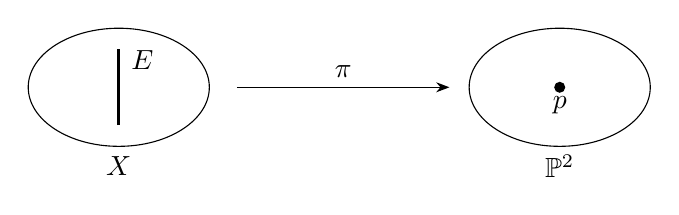
\begin{tikzpicture}[>=Stealth]
\draw (-3.4,0) ellipse (1.15 and .75);
\draw[very thick] (-3.4,-.48)--(-3.4,.48);
\node at (-3.1,.35) {\(E\)};
\node at (-3.4,-1) {\(X\)};
\draw[->] (-1.9,0)--(.8,0) node[midway,above] {\(\pi\)};
\draw (2.2,0) ellipse (1.15 and .75);
\fill (2.2,0) circle (2pt) node[below] {\(p\)};
\node at (2.2,-1) {\(\Pj^2\)};
\end{tikzpicture}
\end{center}
\[
L\cdot E=0,\qquad L^2=1,\qquad
h^0(X,L^m)=\binom{m+2}{2}.
\]
The exceptional curve has degree zero. The picture is schematic.
\end{frame}

\begin{frame}{Kawamata--Viehweg vanishing}
For a nef and big line bundle \(L\) on smooth projective \(X\),
\[
\boxed{H^q(X,K_X\otimes L)=0,\qquad q>0.}
\]
\par\bigskip
\textbf{Kawamata--Viehweg:} obtain vanishing under the weaker positivity assumptions \textquotedblleft nef and big.\textquotedblright
\par\bigskip
\par We will construct a positive singular metric with \(\cI_h=\cO_X\).
\end{frame}

\begin{frame}{The metric construction}
\begin{enumerate}
\setlength{\itemsep}{15pt}
\item Bigness provides an ample part and an effective divisor.
\item Nefness lets us take larger powers without changing that divisor.
\item A large root makes the divisor's singularity integrable.
\end{enumerate}
\par\bigskip
Then apply Nadel.
\end{frame}

\begin{frame}{Bigness provides an ample part}
Fix a smooth very ample divisor \(A\).
\[
h^0(X,L^m)\ge c\,m^n
\quad\text{along a subsequence},\qquad
h^0(A,L^m|_A)=O(m^{n-1}).
\]
There must be a nonzero section vanishing along \(A\).
\[
\boxed{L^d\simeq\cO_X(A+D),\qquad D\ge0.}
\]
This is Kodaira's lemma in the form we need.
\end{frame}

\begin{frame}{Nefness keeps the ample part positive}
Keep \(D\) fixed and increase \(N>d\):
\[
L^N=
\underbrace{L^{N-d}\otimes\cO_X(A)}_{M_N\text{ is ample}}
\otimes\cO_X(D).
\]
We use the projective fact: nef plus ample is ample.
\par\bigskip
\par Give \(M_N\) a smooth positive metric \(h_N\).
\end{frame}

\begin{frame}{An effective divisor supplies positive curvature}
If \(D\) has local equation \(f_D=0\), its divisor metric has weight
\[
h_D=|f_D|^{-2}.
\]
Poincaré--Lelong gives
\[
\boxed{i\Theta_{h_D}=2\pi[D]\ge0.}
\]
The curvature is concentrated along the divisor.
\end{frame}

\begin{frame}{Taking a root makes the singularity milder}
On \(L\), use \(h=(h_Nh_D)^{1/N}\).
Then
\[
i\Theta_h=\frac1N i\Theta_{h_N}+\frac{2\pi}{N}[D]>0.
\]
Locally,
\[
h=(\text{smooth factor})\,|f_D|^{-2/N}.
\]
The divisor is fixed. Its exponent tends to zero.
\end{frame}

\begin{frame}{A mild pole is integrable}
\begin{columns}[c]
\column{.45\textwidth}
\centering
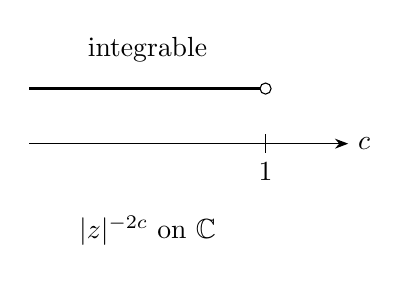
\begin{tikzpicture}[>=Stealth,x=3cm,y=1cm]
\draw[->] (0,0)--(1.35,0) node[right] {\(c\)};
\draw (1,.12)--(1,-.12) node[below] {\(1\)};
\draw[very thick] (0,.7)--(1,.7);
\draw[fill=white] (1,.7) circle (2pt);
\node at (.5,1.2) {integrable};
\node at (.5,-1.1) {\(|z|^{-2c}\) on \(\C\)};
\end{tikzpicture}
\column{.52\textwidth}
\[
\int_0^\delta r^{1-2c}\,dr<\infty
\quad\Longleftrightarrow\quad c<1.
\]
For any nonzero holomorphic \(f\), sufficiently small \(c>0\) makes \(|f|^{-2c}\) locally integrable.
\end{columns}
\medskip
Compactness gives one sufficiently large \(N\) for our fixed \(D\).
\end{frame}

\begin{frame}{Kawamata--Viehweg: conclusion}
The weight of \(h\) is locally integrable, so \(1\in\cI_h\).
Thus
\[
\cI_h=\cO_X.
\]
Nadel now gives
\[
\boxed{H^q(X,K_X\otimes L)=0,\qquad q>0.}
\]
We have reached the second destination.
\end{frame}

\begin{frame}{An older theorem through a newer one}
\begin{center}
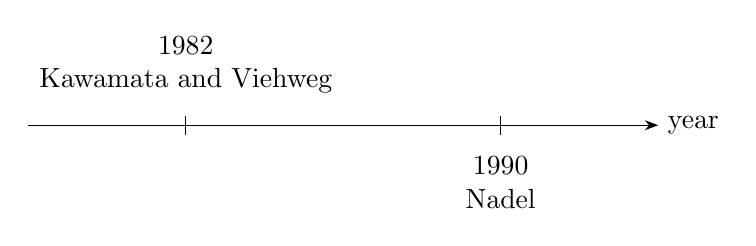
\begin{tikzpicture}[>=Stealth]
\draw[->] (-4,0)--(4,0) node[right] {year};
\draw (-2,.12)--(-2,-.12);
\node[above=8pt,align=center] at (-2,0) {1982\\Kawamata and Viehweg};
\draw (2,.12)--(2,-.12);
\node[below=8pt,align=center] at (2,0) {1990\\Nadel};
\end{tikzpicture}
\end{center}
\par\bigskip
Our proof uses the later analytic theorem to recover the earlier vanishing result.
\src{Kawamata, \emph{Math. Ann.} 261 (1982); Viehweg, \emph{J. reine angew. Math.} 335 (1982); Nadel, \emph{Annals} 132 (1990).}
\end{frame}

\begin{frame}{What the two applications have in common}
\begin{center}
\renewcommand{\arraystretch}{1.8}
\begin{tabular}{lll}
Metric & Ideal & Conclusion\\
\hline
Chosen logarithmic poles & \(\mathfrak m_x,\ \mathfrak m_x^2,\ldots\) & sections give an embedding\\
Mild divisor poles & \(\cO_X\) & ordinary vanishing
\end{tabular}
\end{center}
\par\bigskip
Positive curvature gives vanishing.
The singularities decide which ideal appears.
\end{frame}
\end{document}
